\documentclass{amsart}
\synctex=1

%=================================================================
% 
\newcount\DraftStatus  % 0 suppresses notes to selves in text
\DraftStatus=1   % TODO: set to 0 for final version
%=================================================================

%=================================================================
\usepackage{comment}
%=================================================================
%
\includecomment{JournalOnly}  
\includecomment{ConferenceOnly}  
\includecomment{TulipStyle}
%
%=================================================================
%=================================================================
% gitlatexdiff
%
%  https://gitlab.com/git-latexdiff/git-latexdiff
%=================================================================
%  git latexdiff HEAD  HEAD~5 --main templatex.tex
%  git latexdiff HEAD~1  --main templatex.tex
%  View pdf to see difference
%
%=================================================================
%
% Todo Notes for marginal comments
% 
%\newcount\DraftStatus  % 0 suppresses notes to selves in text
%\DraftStatus=1   % TODO: set to 0 for final version
\ifnum\DraftStatus=1
	\usepackage[draft,colorinlistoftodos,color=orange!30]{todonotes}
\else
	\usepackage[disable,colorinlistoftodos,color=blue!30]{todonotes}
\fi 
%\usepackage[disable]{todonotes} % notes not showed
%\usepackage[draft]{todonotes}   % notes showed
%
\makeatletter
 \providecommand\@dotsep{5}
 \def\listtodoname{List of Todos}
 \def\listoftodos{\@starttoc{tdo}\listtodoname}
 \makeatother
%
%=================================================================
%
\usepackage{color}
\newcommand{\draftnote}[3]{ 
	\todo[author=#2,color=#1!30,size=\footnotesize]{\textsf{#3}}	}
% TODO: add yourself here:
%
\newcommand{\gangli}[1]{\draftnote{blue}{GLi:}{#1}}
\newcommand{\qwu}[1]{\draftnote{red}{QWu:}{#1}}
\newcommand{\gliMarker}
	{\todo[author=GLi,size=\tiny,inline,color=blue!40]
	{Gang Li has worked up to here.}}
\newcommand{\qwuMarker}
	{\todo[author=QWu,size=\tiny,inline,color=red!40]
	{Qiong Wu has worked up to here.}}
%=================================================================

%=================================================================
%
% general packages
%  https://en.wikibooks.org/wiki/Category:Book:LaTeX
%  https://en.wikibooks.org/wiki/LaTeX/Package_Reference
%
%=================================================================
\usepackage{graphicx}
\usepackage{algorithm}
\usepackage{algorithmic}
\usepackage{breqn}
\usepackage{subcaption}
\usepackage{multirow}
\usepackage{psfrag}
\usepackage{url}
\usepackage{hyperref}
%\usepackage[colorlinks]{hyperref}
%\usepackage{cite}
\usepackage{cleveref}
\usepackage{booktabs}
\usepackage{rotating}
\usepackage{colortbl}
\usepackage{paralist}
%\usepackage{geometry}
\usepackage{epstopdf}
\usepackage{nag}
\usepackage{microtype}
\usepackage{siunitx}
\usepackage{nicefrac}
% for random text
\usepackage{lipsum}
\usepackage[english]{babel}
\usepackage[pangram]{blindtext}
% for tikz figures
\usepackage{tikz}
\usetikzlibrary{fit,positioning,arrows.meta,shapes,arrows}
%\tikzset{neuron/.style={circle,thick,fill=black!25,minimum size=17pt,inner sep=0pt},
%	input neuron/.style={neuron, draw,thick, fill=gray!30},
%	hidden neuron/.style={neuron,fill=white,draw},
%	hoz/.style={rotate=-90}}
%
%=================================================================



\begin{TulipStyle}
\usepackage{natbib}
%=================================================================
%
% Version control information
%
%=================================================================
\usepackage{gitinfo2}
%=================================================================
\usepackage{fancyhdr}
\pagestyle{fancy}
\fancyhead{} % clear all header fields
\fancyhead[RO,LE]{\textsl{\rightmark}}
\fancyhead[LO,RE]{\ensuremath{\Rightarrow}
		\textbf{\textbf{[CONFIDENTIAL]}}\ensuremath{\Leftarrow}}
\fancyhead[CO,CE]{}
%=================================================================
\fancyfoot{} % clear all footer fields
\fancyfoot[CE,CO]{\textbf{\thepage}} 
\fancyfoot[LO,LE]{
\includegraphics[height=.9\headheight]{logos/tulip-logo.eps}
		\gitVtagn-\gitBranch\ (\gitCommitterDate)}
\fancyfoot[RO,RE]{Committed by: \textsl{\gitCommitterName}}

\setlength{\headheight}{12pt}
\renewcommand{\headrulewidth}{0.4pt}
\renewcommand{\footrulewidth}{0.4pt}
%=================================================================


%=================================================================
% for math notations
% ----------------------------------------------------------------
\usepackage{mathtools}
\usepackage{amsthm}
%
% THEOREMS -------------------------------------------------------
%
\newtheorem{thm}{Theorem}[section]
\newtheorem{cor}[thm]{Corollary}
\newtheorem{lem}[thm]{Lemma}
\newtheorem{prop}[thm]{Proposition}
\theoremstyle{definition}
\newtheorem{defn}[thm]{Definition}
\theoremstyle{remark}
\newtheorem{rem}[thm]{Remark}
\numberwithin{equation}{section}
% MATH -----------------------------------------------------------
\newcommand{\norm}[1]{\left\Vert#1\right\Vert}
\newcommand{\abs}[1]{\left\vert#1\right\vert}
\newcommand{\set}[1]{\left\{#1\right\}}
\newcommand{\Real}{\mathbb R}
\newcommand{\eps}{\varepsilon}
\newcommand{\To}{\longrightarrow}
\newcommand{\BX}{\mathbf{B}(X)}
% ----------------------------------------------------------------
\newcommand{\I}{{\cal I}}
\newcommand{\Id}{{\cal I} }
\newcommand{\Dc}{{\cal D}}
\newcommand{\J}{{\cal J}}
\newcommand{\Dn}{{\cal D}_n}
\newcommand{\Dd}{{\cal D}_n }
\renewcommand{\P}{{\cal P}}
\newcommand{\Nu}{{\cal N} }
\newcommand{\B}{{\cal B}}
\newcommand{\Bf}{{\bf B}}
\newcommand{\Y}{{\bf Y}}
\newcommand{\A}{{\cal A}}
% ----------------------------------------------------------------
\newcommand{\V}{{\cal V}}
\newcommand{\M}{{\cal M}}
\newcommand{\F}{{\cal F}}
\newcommand{\Fd}{{\cal F}}
\newcommand{\BF}{{\cal BF}_n}
\newcommand{\BFd}{{\cal BF}_n}
\newcommand{\TF}{{\cal TF}_n}
\newcommand{\TFd}{{\cal TF}_n}
%\newcommand{\G}{{\cal G}}
\newcommand{\X}{{\cal X}}
\newcommand{\E}{{\cal E}}
\newcommand{\K}{{\cal K}}
\newcommand{\T}{{\cal T}_n}
\renewcommand{\H}{{\cal H}}
% ----------------------------------------------------------------
\newtheorem{Remark}{Remark}
\newtheorem{proposition}{Proposition}
\newtheorem{theorem}{Theorem}
\newtheorem{lemma}{Lemma}
\newtheorem{corollary}{Corollary}
\newtheorem{example}{Example}
\newtheorem{definition}{Definition}
\newtheorem{Algorithms}{Algorithm}
% ----------------------------------------------------------------
\newcommand{\bu}{{\mathbf 1} }
\newcommand{\bo}{{\mathbf 0} }
\newcommand{\N}{\mbox{{\sl l}}\!\mbox{{\sl N}}}
% ----------------------------------------------------------------
\def\uint{[0,1]}
\def\proof{{\scshape Proof}. \ignorespaces}
\def\endproof{{\hfill \vbox{\hrule\hbox{%
   \vrule height1.3ex\hskip1.0ex\vrule}\hrule
  }}\par}
%
%=================================================================

\hypersetup
{
    pdfauthor={\gitAuthorName},
    pdfsubject={TULIP Lab},
    pdftitle={},
    pdfkeywords={TULIP Lab, Data Science},
%	bookmarks=true,  
}

\end{TulipStyle}




%=================================================================
%
\begin{document}
%
%=================================================================
%
\title[FLIP01 Report]{FLIP01 Final-term Report}%

\author{Jiahui ZHou}
\address[A.~1]{School of Computer Science,\\ 
Xi'an Shiyou University, Shaanxi 710065, China}%
\email[A.~1]{rukamihara@outlook.com}

%\thanks{Thanks to \ldots}%
\subjclass{Natual Language Processing}%
\keywords{Multi-task Regression, Text Processing, Question\&Anewser, ...}%
\date{\gitAuthorDate}%

\begin{abstract}
The abstract will be put here, ....
\end{abstract}

\maketitle
\tableofcontents

\newpage
%=================================================================

%=================================================================
\section{Introduction}\label{sec-intro}
\subsection{Problem Statement}
The competation \textit{Google QUEST Q\&A Labeling} is designed to 
improving automated understanding of complex question answer content.
The challenge is to use this new dataset to build predictive algorithms for different subjective aspects of question-answering. 
The question-answer pairs were gathered from nearly 70 different websites, in a "common-sense" fashion.
\begin{figure}[htbp]
    \centering
    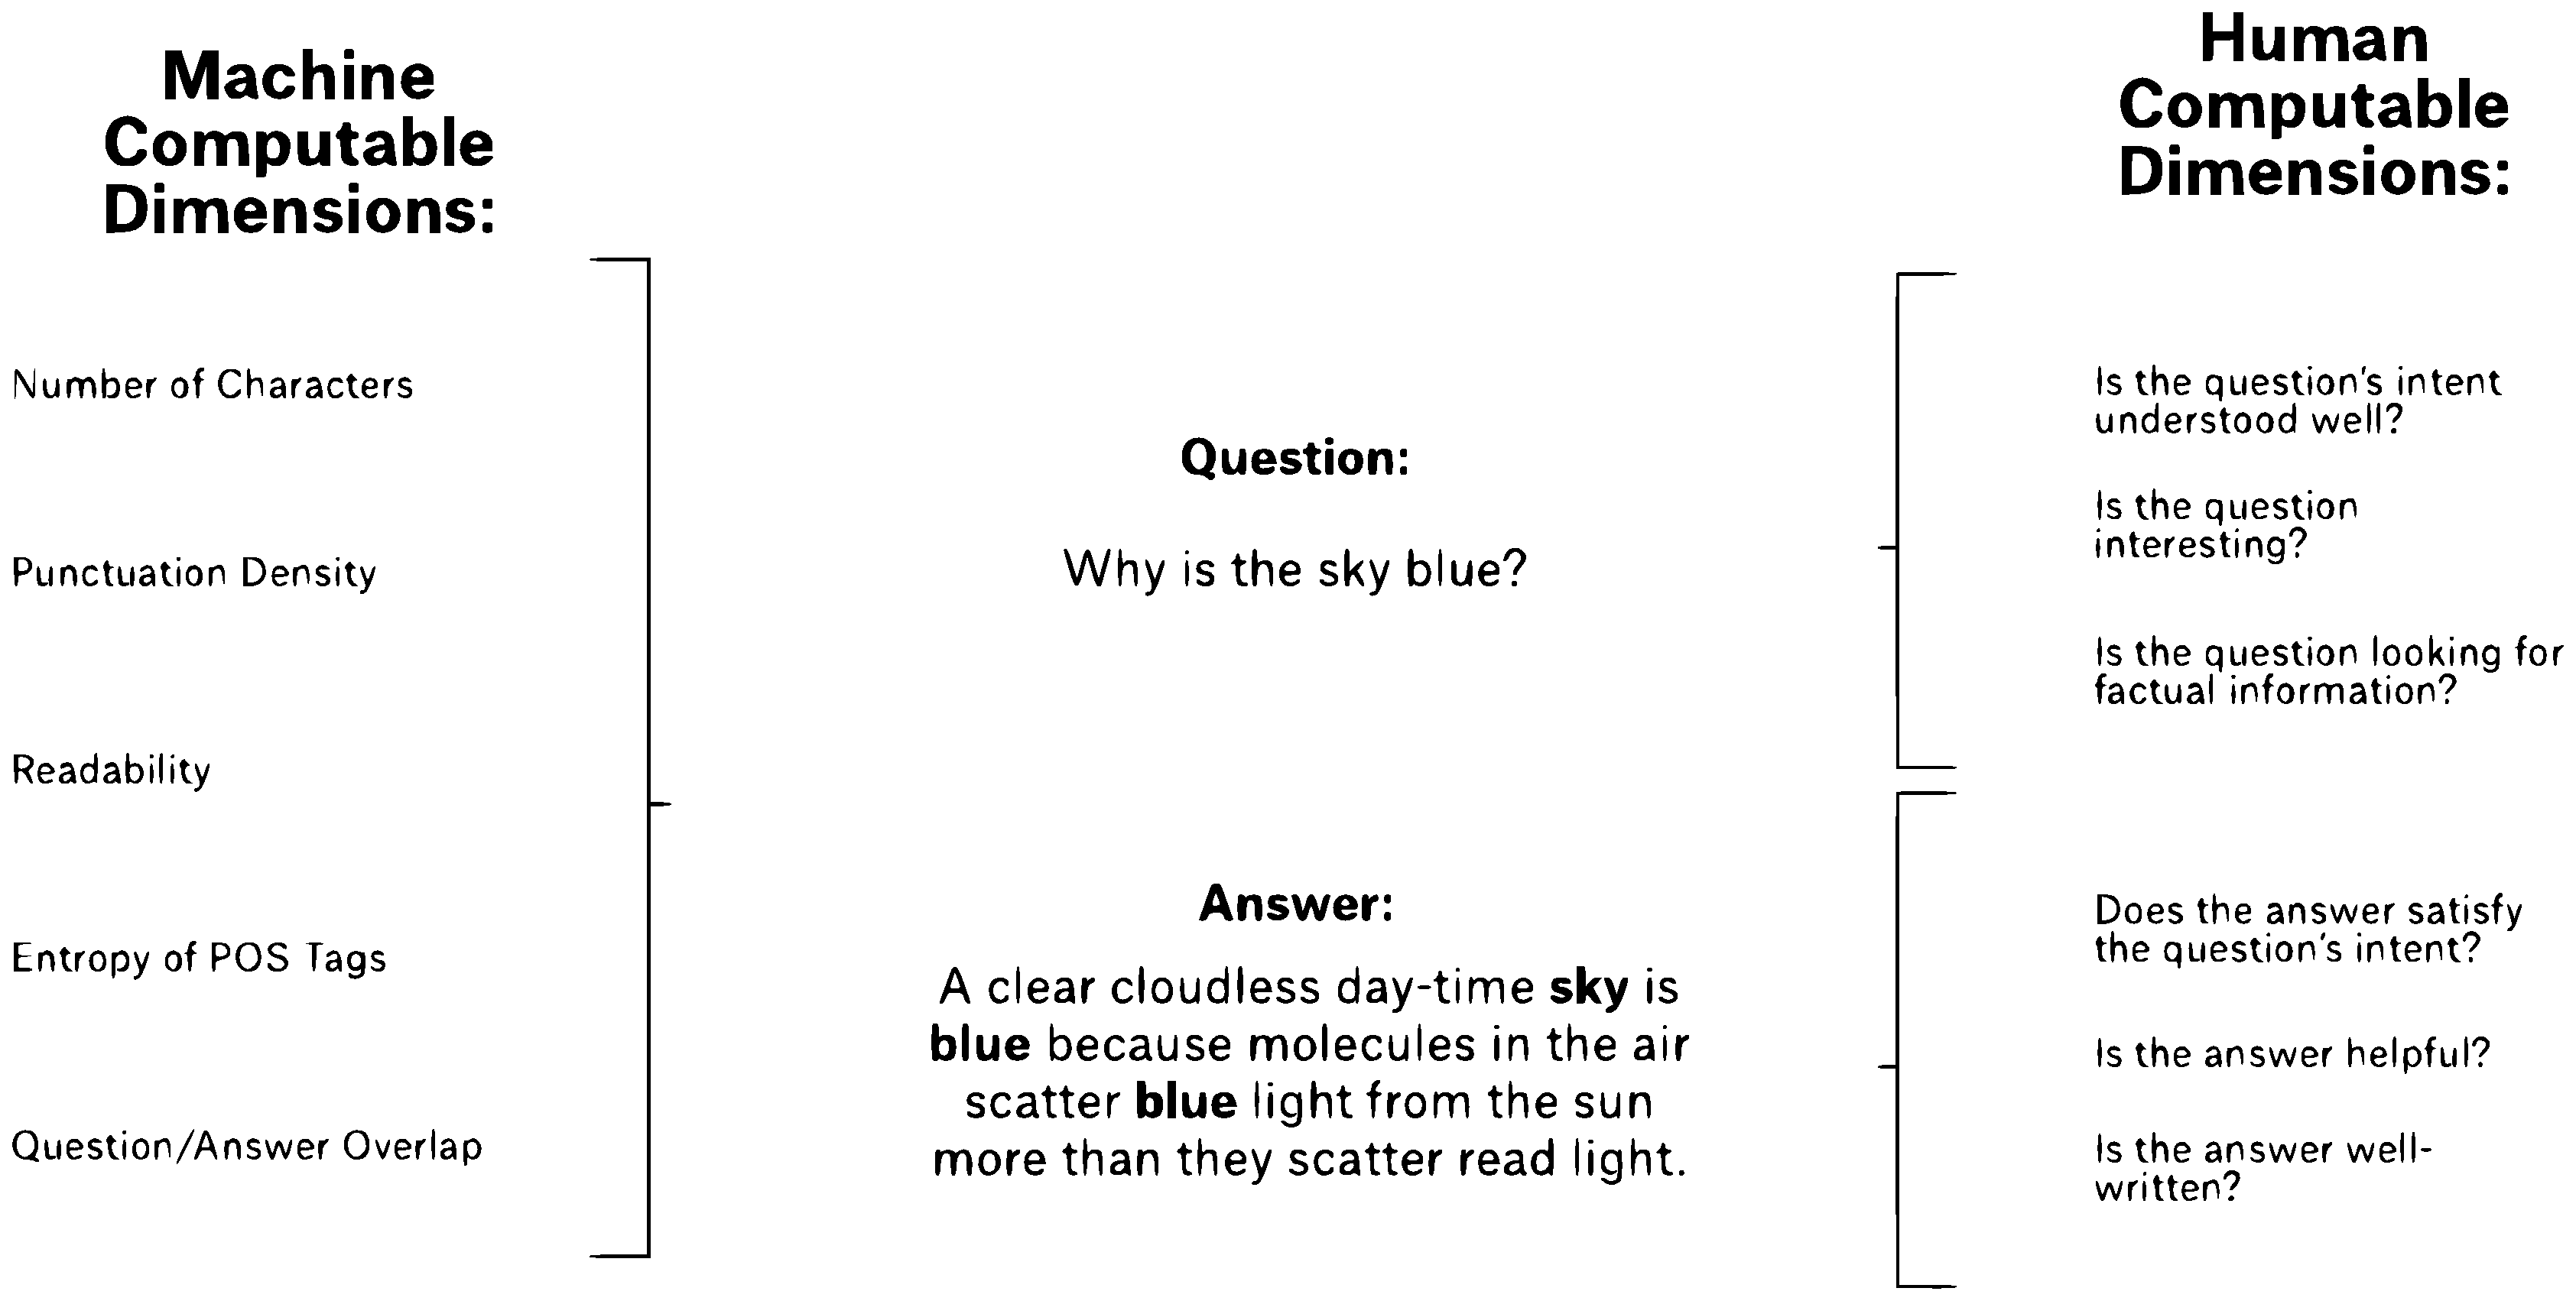
\includegraphics[width=30em]{figures/title.eps}
    \caption{Different between machine and human answer}
    \label{fig:title}
\end{figure}
\subsection{Dataset}
The dataset contains 6049 records in training set and 476 records in test set, with the following features:
\begin{itemize}
    \item Question title\&body
    \item Answer
    \item Host
    \item Category
    \item Question user
    \item Answer user
    \item Url
\end{itemize}
The targets are both continuous values in the range of $[0,1]$, representing the score of this record in the corrsponding dimension.
It contains 21 question related targets and 9 answer related targets.

\subsection{Solution}
Transformer Models such as \textit{Bert} are proven have great performance on many nlp tasks, especially for Question\&Anwser tasks.
In this competation, I will use Bert Model to solve the problem.
\newpage
\section{EDA and Data Preprocessing} \label{sec-eda}
\subsection{Category}
The QA pairs is collected from over 70 different web site,with 7 different category.
\begin{figure}[htbp]
    \centering
    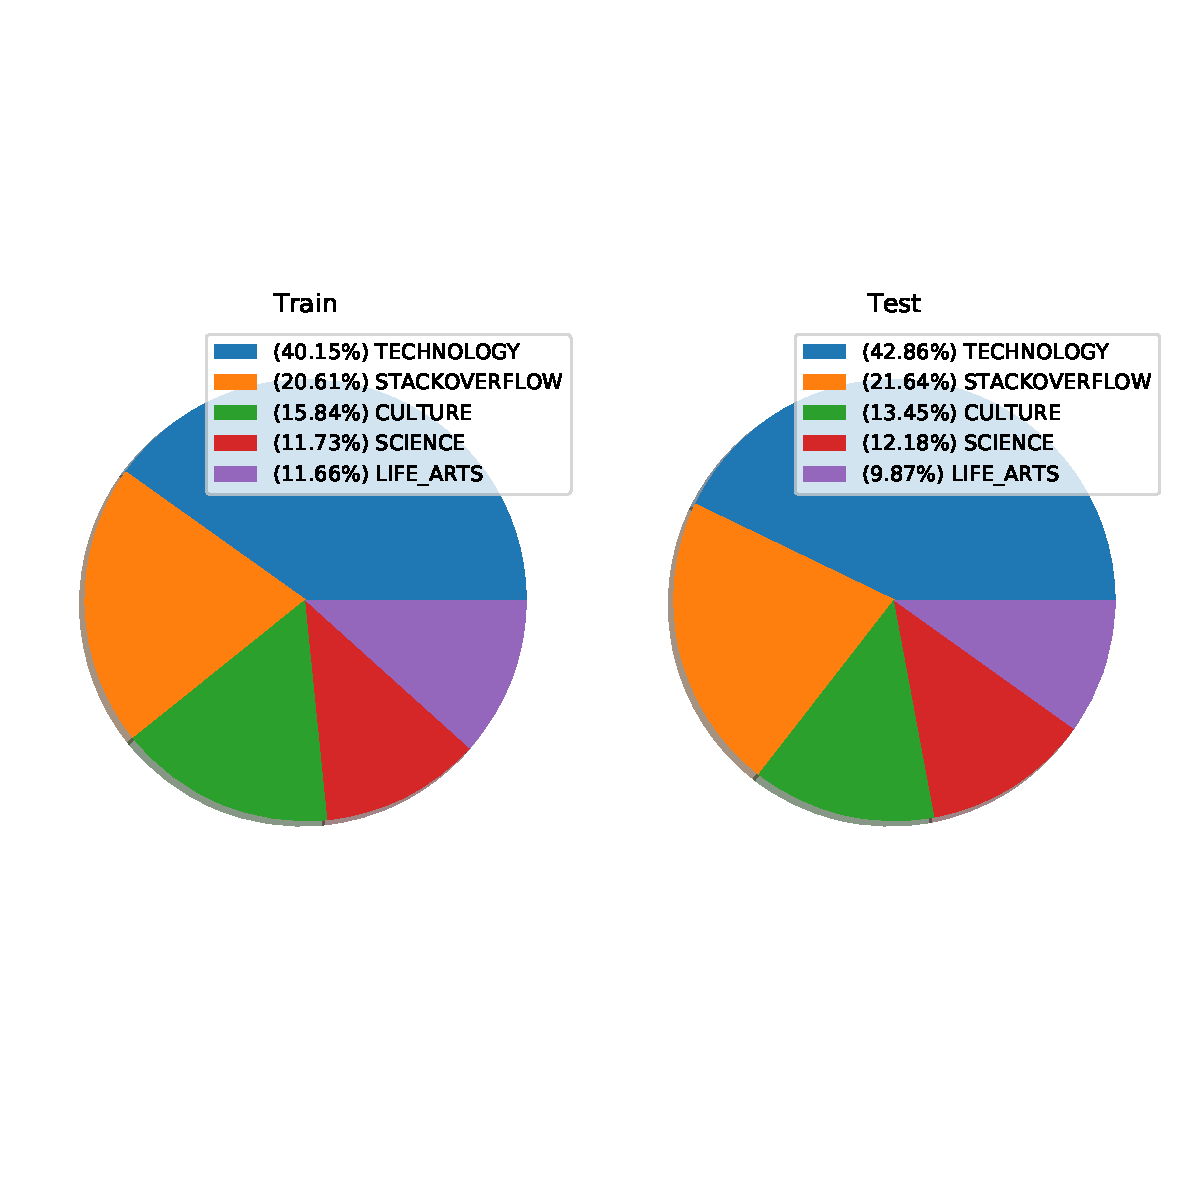
\includegraphics[width=.5\linewidth]{figures/categories.pdf}
    \caption{Category Distribution}
    \label{fig:categories}
\end{figure}
\subsection{Targets}
The 30 targets shoud be continuous values according to the competition description.
But in fact, according to the training set, they have only several fixed values.
\begin{figure}[htbp]
    \centering
    \centering
    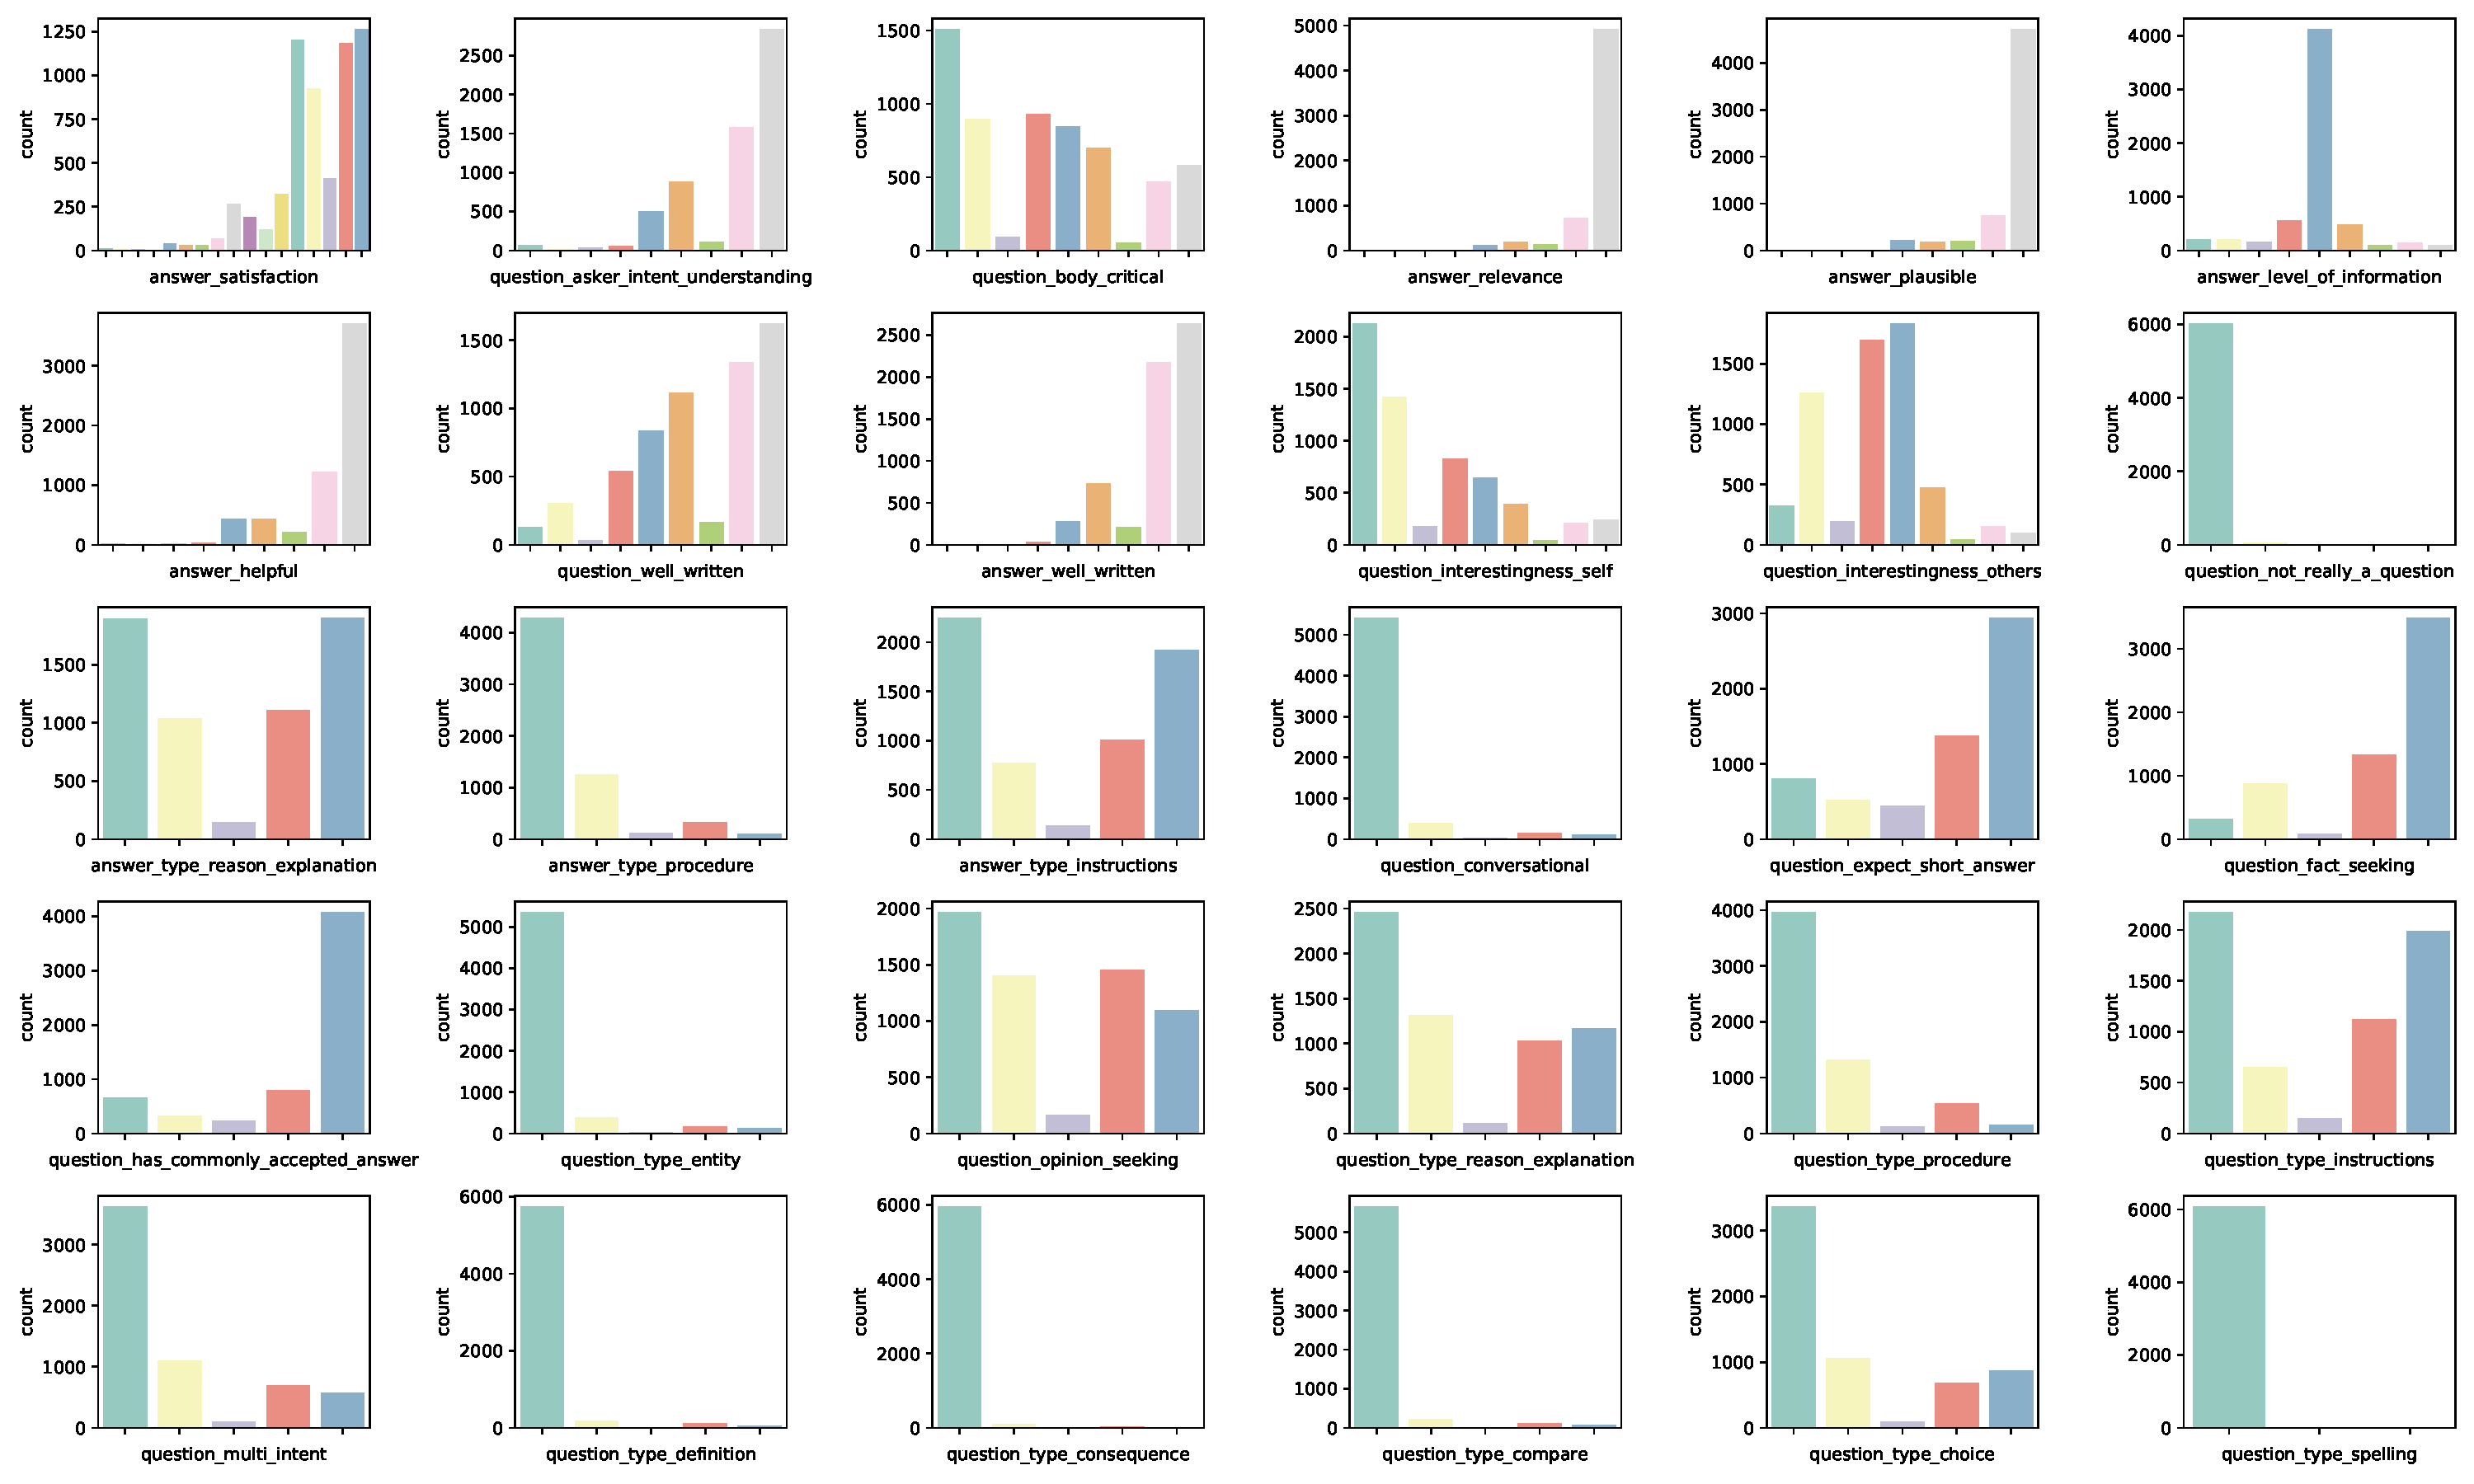
\includegraphics[width=\linewidth]{figures/targets.pdf}
    \caption{Targets Distribution}
    \label{fig:targets}
\end{figure}

The box plot below shows the corresponding between target values and categories. 
It's interesting to notice that:
\begin{itemize}
    \item Target distribution alone categories have not much different.
    \item Some targets have a very sharp distribution.
\end{itemize}
\begin{figure}[htbp]
    \centering
    \centering
    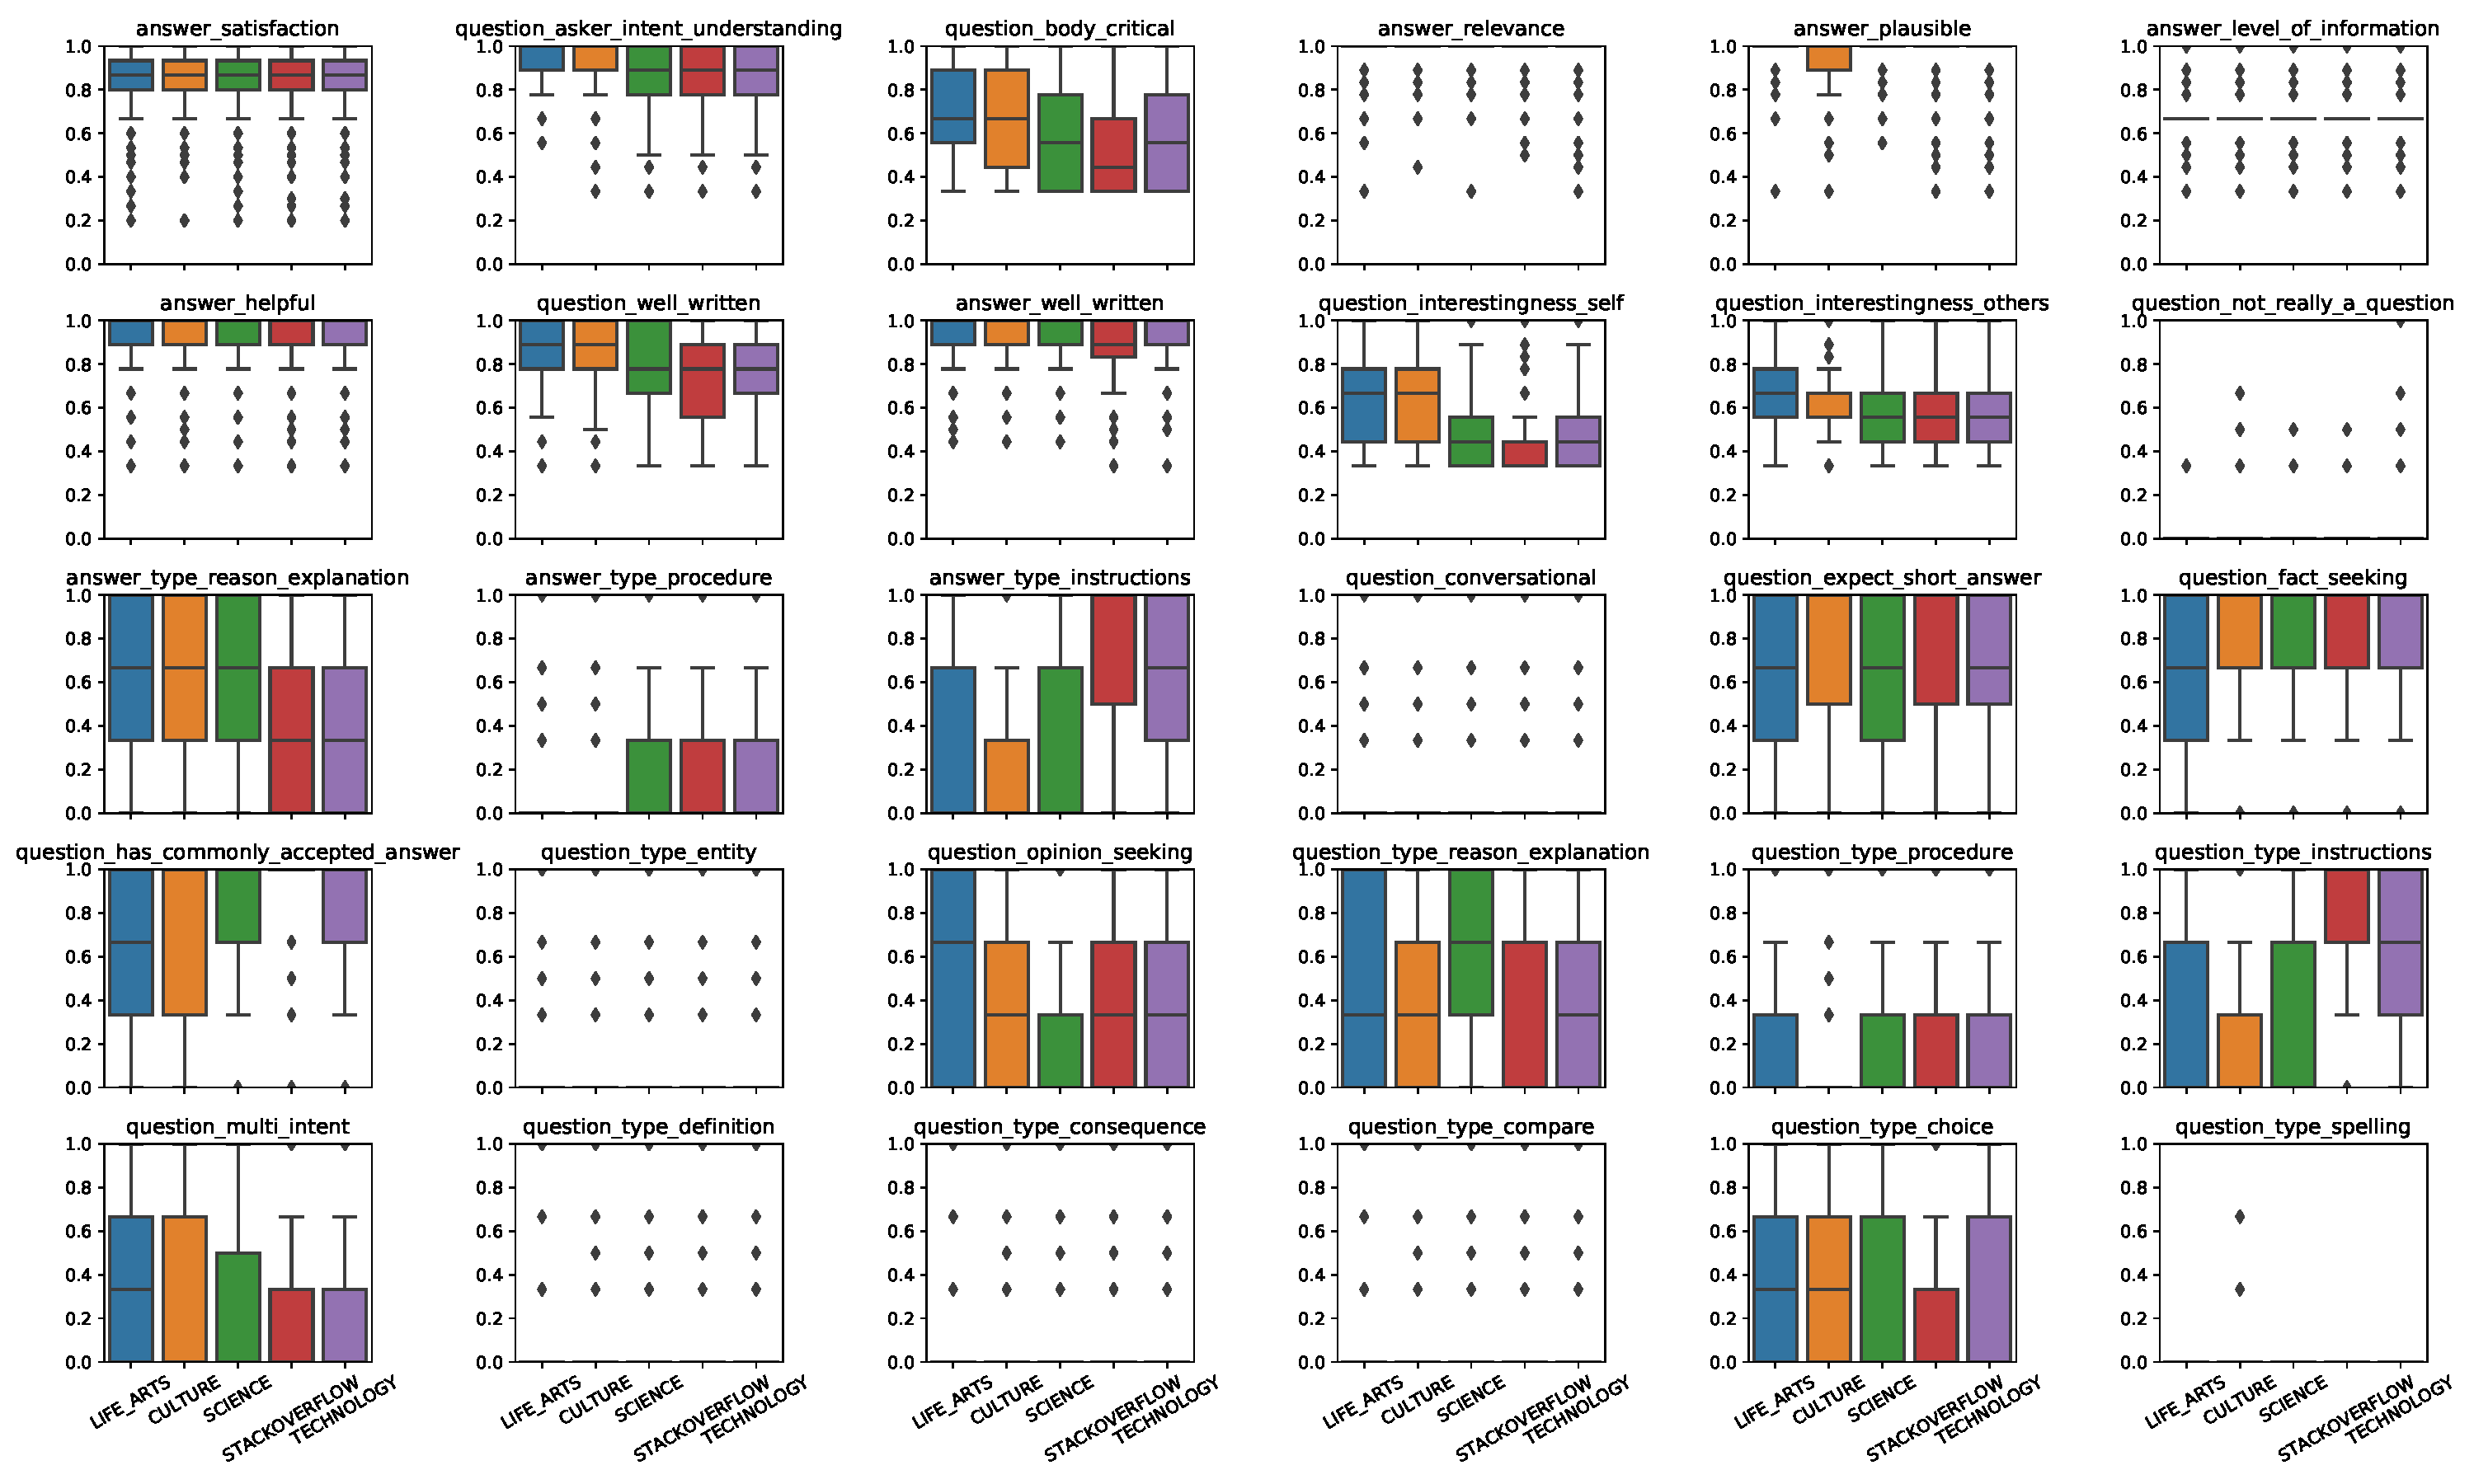
\includegraphics[width=\linewidth]{figures/target_category_distribution.pdf}
    \caption{Targets Distribution}
    \label{fig:targets}
\end{figure}
\subsection{Duplicated Questions}
The competition description has said that:
\begin{itemize}
    \item \emph{The training data contains rows with some duplicated questions (but with different answers). }
    \item \emph{The test data does not contain any duplicated questions.}
\end{itemize}
\begin{table}[htbp]  
    \centering
    \caption{Duplicated Questions}
    \label{tbl:dup_q}
    \begin{tabular}{lc}
        \hline
        Question Title & Count \\
        \hline
        What is the best introductory Bayesian statist...   &12\\
        Important non-technical course for programmers?	    &11\\
        What does mathematics have to do with programm...   &11\\
        How to prevent the "Too awesome to use" syndrome    & 9\\
        How do I deal with a slow and undedicated coll...   & 7\\
        No sound in Ubuntu except at log in	                & 7\\
        What are the benefits of owning a physical book?    & 7\\
        Another instructor is pushing me out of the cl...   & 7\\
        Does "so far, so good" carry a negative connot...   & 6\\
        Good travel games for two players, especially ...   & 6\\
        \dots&-\\
        \hline
    \end{tabular}
\end{table}
\begin{itemize}
    \item The question related targets of these records are not always equle.
    \item It's reasonable to set all question related targets of duplicated questions to its mode or mean.
    \begin{itemize}
        \item \emph{t1:\ question_asker_intent_understanding}
        \item \emph{t2:\ question_body_critical}
        \item \emph{t3:\ question_conversational}
    \end{itemize}
\end{itemize}
    \begin{table}
        \centering
        \caption{The same question-related target of duplicated questions should have the same value in order to reach a better result.}
        \label{tbl:dp_before}
        \begin{minipage}{0.48\linewidth}
        \begin{tabular}{cccc}
            \hline
            qa_id	&t1 &t2 &t3 \\
            \hline
            366	    &1.00000 &1.00000 &0.00000\\
            2536	&1.00000 &1.00000 &0.66667\\
            2591	&1.00000 &1.00000 &1.00000\\
            3349	&1.00000 &1.00000 &1.00000\\
            5543	&1.00000 &1.00000 &0.00000\\
            5989	&1.00000 &1.00000 &1.00000\\
            6041	&0.77778 &1.00000 &0.66667\\
            6215	&1.00000 &0.88889 &0.33333\\
            7003	&0.77777 &1.00000 &1.00000\\
            8328	&1.00000 &1.00000 &0.66667\\
            8867	&1.00000 &1.00000 &0.66667\\
            9137	&1.00000 &1.00000 &0.00000\\
            \hline
        \end{tabular}
    \end{minipage}
    \begin{minipage}{0.48\linewidth}
        \begin{tabular}{cccc}
            \hline
            qa_id	&t1 &t2 &t3 \\
            \hline
            366	    &1.00000 &1.00000 &0.66667\\
            2536	&1.00000 &1.00000 &0.66667\\
            2591	&1.00000 &1.00000 &0.66667\\
            3349	&1.00000 &1.00000 &0.66667\\
            5543	&1.00000 &1.00000 &0.66667\\
            5989	&1.00000 &1.00000 &0.66667\\
            6041	&1.00000 &1.00000 &0.66667\\
            6215	&1.00000 &1.00000 &0.66667\\
            7003	&1.00000 &1.00000 &0.66667\\
            8328	&1.00000 &1.00000 &0.66667\\
            8867	&1.00000 &1.00000 &0.66667\\
            9137	&1.00000 &1.00000 &0.66667\\
            \hline
        \end{tabular}
    \end{minipage}
    \end{table}
\section{Method} \label{sec-method}
BERT is a deep learning model that has given state-of-the-art results on 
a wide variety of natural language processing tasks. 
It stands for \textbf{Bidirectional Encoder Representations for Transformers.}
It has been pre-trained on Wikipedia and BooksCorpus and requires (only) task-specific fine-tuning.

The fine-tune of BERT requires a series of text preprocessing, include wordpiece tokenization and 
three different embedding。
\subsection{Wordpiece Tokenization}
The wordpiece model chooses the two tokens to combine that 
would give the training corpus the highest probability.
Rather than merging the pairs that are most frequent, 
wordpiece instead merges the pairs that minimizes 
the language model likelihood of the training data.

The intuition of wordpiece tokenization is:
\begin{itemize}
    \item First, Split input sentence using some simple basic tokenizer (like whitespace) into a series of rough word tokens.
    \item Then word-initial subwords are distinguished from those that do not start words by marking internal subwords with special symbols \#\#
    \item Finally, tokenize every word token string using a greedy longest-match-first algorithm.
\end{itemize}

The greedy longest-match-first algorithm used here is also called \emph{MaxMatch} algorithm.
\begin{algorithm}[htbp]
	\small
	\caption{MaxMatch Algorithm}
	\label{alg:maxmatch}
	\begin{algorithmic}[1]
		\REQUIRE
        string to be tokenize $string$,
        The vocabulary $dic$
		\ENSURE
        list of tokens $T$.
        \IF{$string is empty$}
        \RETURN $empty list$
        \ENDIF
        \FOR {$i\leftarrow length(sentence) $\textbf{downto} $1$}
        \STATE $firstword$ = first $i$ chars of sentence
        \STATE $remainder$ = rest of sentence
        \IF{InDictionary($firstword,dict$)}
        \RETURN list($firstword$, MaxMatch($remainder, dict$))
        \ENDIF
        \ENDFOR
	\end{algorithmic}
\end{algorithm}
\subsection{Embedding}
The idea of vector semantics is thus to represent a word as a point in some multidimensional semantic space.
Vectors for representing words are generally called embeddings, because the word is embedded in a particular vector space.
After convert to embeddings, words with similar meanings are nearby in space.

There are two commonly used vector semantic models. tf-idf and word2vec.
\subsubsection{Tf-idf}
The tf-idf algorithm is the product
of two terms, each term capturing one of these two intuitions:
The first is the \textbf{term frequency}:the frequency of the word $t$ in the
document $d$. We can just use the raw count as the term frequency:
\begin{equation}
    tf_{t,d}=count(t,d)
\end{equation}
The second is used to give a higher weight to words that occur only in a
document frequency few documents,called the \textbf{inverse document frequency}. 
The document frequency $df_t$ of a term $t$ is the number of documents it occurs in.
\begin{equation}
    idf_t = \log_{10}{(\frac{N}{df_t})}
\end{equation}
Then we get the tf-idf weight value:
\begin{equation}
    w_{t,d}=tf_{d,f}\times idf_t
\end{equation}
The tf-idf vector model represents a target word as a vector with dimensions 
corresponding to all the words in the vocabulary (length $|V|$, with vocabularies of 20,000 to 50,000).
The values in each dimension are the frequency with which the target 
word co-occurs with each neighboring context word, weighted by tf-idf.
It can also be used to represent a document by the centroid document vector.
Given $k$ word vectors $w_1, w_2, \dots, w_k$, the centroid document vector $d$ is:
\begin{equation}
    d = \frac{w_1+w_2+\dots+w_k}{k}
\end{equation}
The vector can be used to estimate the similarity between the two word or documents by
compute $\cos{(d_1, d_2)}$.

\subsubsection{Word2vec}
The tf-idf vector model represent a word as a sparse, long vector. 
And it can't capture the words'position information. 
To do this, the word2vec algorithm is a better choice.
It also represent words as very short, dense vectors. 
It turn out that dense vectors work better in every NLP task than sparse vectors.

The skip-gram algorithm is one of two algorithms in a software package called word2vec,
and so sometimes the algorithm is loosely referred to as word2vec. The intuition of word2vec is that
given tuple $(t, c)$ of target word $t$ and candidate context word $c$, get whether $c$ is a real context word. (binary classification)

The intuition of skip-gram is:
\begin{enumerate}
    \item Treat the target word and a neighboring context word as positive examples.
    \item Randomly sample other words in the lexicon to get negative samples.
    \item Use logistic reg to train a classifier to distinguish those two cases.
    \item Use the reg weights as the embeddings.
\end{enumerate}
\subsubsection{WordPiece}

\subsection{Transformer}
\subsection{BERT}

\section{Experiment and Analysis} \label{sec-experiment}
\subsection{Model Building}
\subsection{Experiment}
\section{Conclusions} \label{sec-conclusions}


The authors would like to thank \ldots



% ----------------------------------------------------------------
\newpage
\bibliography{tuliplab,yourbib}
\bibliographystyle{plain}
%=================================================================

\listoftodos

\end{document}

